%%%%%%%%%%%%%%%%%%%%%%%%%%%%%%%%%%%%%%%%%
% Beamer Presentation
% LaTeX Template
% Version 1.0 (10/11/12)
%
% This template has been downloaded from:
% http://www.LaTeXTemplates.com
%
% License:
% CC BY-NC-SA 3.0 (http://creativecommons.org/licenses/by-nc-sa/3.0/)
%
%%%%%%%%%%%%%%%%%%%%%%%%%%%%%%%%%%%%%%%%%

%----------------------------------------------------------------------------------------
%	PACKAGES AND THEMES
%----------------------------------------------------------------------------------------

\documentclass{beamer}

\mode<presentation> {

% The Beamer class comes with a number of default slide themes
% which change the colors and layouts of slides. Below this is a list
% of all the themes, uncomment each in turn to see what they look like.

%\usetheme{default}
%\usetheme{AnnArbor}
%\usetheme{Antibes}
%\usetheme{Bergen}
%\usetheme{Berkeley}
%\usetheme{Berlin}
%\usetheme{Boadilla}
%\usetheme{CambridgeUS}
%\usetheme{Copenhagen}
%\usetheme{Darmstadt}
%\usetheme{Dresden}
%\usetheme{Frankfurt}
%\usetheme{Goettingen}
%\usetheme{Hannover}
%\usetheme{Ilmenau}
%\usetheme{JuanLesPins}
%\usetheme{Luebeck}
\usetheme{Madrid}
%\usetheme{Malmoe}
%\usetheme{Marburg}
%\usetheme{Montpellier}
%\usetheme{PaloAlto}
%\usetheme{Pittsburgh}
%\usetheme{Rochester}
%\usetheme{Singapore}
%\usetheme{Szeged}
%\usetheme{Warsaw}

% As well as themes, the Beamer class has a number of color themes
% for any slide theme. Uncomment each of these in turn to see how it
% changes the colors of your current slide theme.

%\usecolortheme{albatross}
%\usecolortheme{beaver}
%\usecolortheme{beetle}
%\usecolortheme{crane}
%\usecolortheme{dolphin}
%\usecolortheme{dove}
%\usecolortheme{fly}
%\usecolortheme{lily}
%\usecolortheme{orchid}
%\usecolortheme{rose}
%\usecolortheme{seagull}
%\usecolortheme{seahorse}
%\usecolortheme{whale}
%\usecolortheme{wolverine}

%\setbeamertemplate{footline} % To remove the footer line in all slides uncomment this line
%\setbeamertemplate{footline}[page number] % To replace the footer line in all slides with a simple slide count uncomment this line

%\setbeamertemplate{navigation symbols}{} % To remove the navigation symbols from the bottom of all slides uncomment this line
}

\usepackage{graphicx} % Allows including images
\usepackage{subcaption}
\usepackage{booktabs} % Allows the use of \toprule, \midrule and \bottomrule in tables
\usepackage{amsmath}
\usepackage{tikz}
\usepackage{csvsimple}
\usepackage{hyperref}
\hypersetup{
    colorlinks=true,
    linkcolor=blue,
    filecolor=magenta,      
    urlcolor=cyan,
}
\usepackage[
  backend=biber,
  style=apa,
  citestyle=apa
]{biblatex}
\usetikzlibrary{arrows}

\addbibresource{references.bib}

\def\indep{\perp \!\!\! \perp}

%----------------------------------------------------------------------------------------
%	TITLE PAGE
%----------------------------------------------------------------------------------------

\title[Causal Discovery DSGE]{Causal Discovery of DSGE Models} % The short title appears at the bottom of every slide, the full title is only on the title page

\author{Emmet Hall-Hoffarth} % Your name
\institute[Oxford] % Your institution as it will appear on the bottom of every slide, may be shorthand to save space
{
University of Oxford \\ % Your institution for the title page
\medskip
\textit{emmet.hall-hoffarth@economics.ox.ac.uk} % Your email address
}
\date{\today} % Date, can be changed to a custom date

\begin{document}

\begin{frame}
    \titlepage % Print the title page as the first slide
\end{frame}

\section{Overview}

\begin{frame}
    \frametitle{Overview}
    \begin{itemize}
        \item Causal discovery uses algorithms and data to identify causal models.
        \item Suppose that some observed data can be rationalised by some DSGE model. I use some concepts from this literature to provide a test and algorithm to identify the log-linear (state-space) approximation of that model.
        \item Test and algorithm are asymptotically consistent for a unique solution.
        \item Performs well in small sample simulations and real data.
    \end{itemize}
\end{frame}

\section{What?}

\begin{frame}
    \frametitle{DSGE Models}
    \begin{minipage}{0.4\textwidth}
        \centering
        Consumer problem
        \begin{align*}
            & \max \text{ } \sum_{t=0}^{\infty} \beta^t U(C_t, L_t, ...) \text{ } s.t. \\
            & \text{ } P_t C_t + ... \leq W_t L_t + ... \text{ } \forall t \\
            & \lim_{T \rightarrow \infty} \beta^T \lambda_{x,T} x_T \rightarrow 0 \text{ } \forall x \in \{K, B, ...\}
        \end{align*}
    \end{minipage}
    \begin{minipage}{0.4\textwidth}
        \centering
        Firm problem
        \begin{align*}
            \max \text{ } & P_t f(L_t, ...) - W_t L_t - ... \text{ } \forall t \\
        \end{align*}
    \end{minipage}
    \vskip 1cm
    \centering
    Competitive equilibrium, market clearing conditions ...
\end{frame}

\begin{frame}
    \frametitle{State Space Representation}
    \begin{itemize}
        \item Log-linear approximation yields the following general solution: 
    \end{itemize}
        \begin{align}
            \vec{y}_t &= \vec{A} \vec{x}_{t-1} + \vec{B} \vec{z}_{t} \label{ss_solution:x}\\
            \vec{x}_t &= \vec{C} \vec{x}_{t-1} + \vec{D} \vec{z}_{t} \label{ss_solution:y}\\
            \vec{z}_t &= \vec{E} \vec{z}_{t-1} + \vec{\epsilon}_{t} \label{ss_solution:z}
        \end{align}
    \begin{itemize}
        \item Partition variables $\vec{w}_t$ into three categories:
        \begin{itemize}
            \item $\vec{x}_t$: predetermined or endogenous state variables
            \item $\vec{y}_t$: control variables or "jumpers"
            \item $\vec{z}_t$: exogenous state variables
        \end{itemize}
        \item Algorithm identifies partition (and $\vec{A}$ - $\vec{E}$).
    \end{itemize}
\end{frame}

\begin{frame}
    \frametitle{Results (I)}
    \begin{itemize}
        \item Baseline RBC model.
        \item 9 Observables, true partition is $\vec{z} = [g \text{ } z]$, $\vec{x} = [k]$, $\vec{y} = [y \text{ } c \text{ } i \text{ } r \text{ } w \text{ } l]$.
        \item With large sample of $10^6$ observations algorithm uniquely identifies true partition.
        \item 834 models considered (models with $1 \leq$ \# state variables $\leq 3$).
        \item 19683 possible models reduced to just 1.
    \end{itemize}
\end{frame}

\begin{frame}
    \frametitle{Results (II)}
    \begin{itemize}
        \small
        \item 1000 iterations, 100 sample size
        \item Wins = number of times model selected, Valid = number of times model is valid relative to CI test
    \end{itemize}
    \begin{table}
        \centering
        \tiny
        \begin{tabular}{|c|c|c|l|l|}
            \bfseries Index & \bfseries Exogenous States & \bfseries Endogenous States & \bfseries Wins & \bfseries Valid
            \csvreader[head to column names]{./files/rbc_wins_new.csv}{}
            {\\\index & \exostates & \endostates & \wins & \valid}
        \end{tabular}
    \end{table}
\end{frame}

\section{Why?}

\begin{frame}
    \frametitle{Why is this useful?}
    \begin{itemize}
        \item Reduction in the problem space
        \begin{itemize}
            \item Given a set of observations over $k$ variables there are $3^k$ possible state-space partitions. Reduce this to just one (or very small subset).
            \item However, still doesn't reduce to a single structural model (microeconomic dissonance).
        \end{itemize}

        \item Agnosticism
        \begin{itemize}
            \item Assume nothing in particular about each variable --- treat them all the same.
            \item As a result the solution produced reflects the data to the greatest extent possible.
        \end{itemize}

        \item Inference
        \begin{itemize}
            \item Is consumption predetermined? If so then habits important to explain behaviour.
            \item Is inflation predetermined? If so then it is probably not fully rational / forward looking.
        \end{itemize}
        
    \end{itemize}
\end{frame}

\section{How?}

\begin{frame}
    \frametitle{(Massively Oversimplified) Methodology}
    \begin{itemize}
        \item State-Space model is also a DAG, therefore, it implies a set of conditional independence relationships:
    \end{itemize}
    \begin{align}
        x_t \indep x^{\prime}_{t} \,||\,& [\vec{x}_{t-1},\vec{z}_t] \text{ for all } (x_t, x^{\prime}_{t}) \in [\vec{x}_t, \vec{y}_t] \label{constraint_test:1} \\
        x_{t-1} \indep z_{t} \,||\,& \vec{z}_{t-1} \text{ for all } x_{t-1} \in \vec{x}_{t-1} \text{ and } z_{t} \in \vec{z}_t \label{constraint_test:3} \\
        x_t \indep z_{t-1} \,||\,& [\vec{x}_{t-1}, \vec{z}_t] \text{ for all } x_t \in [\vec{x}_t, \vec{y}_t] \text{ and } z_{t-1} \in \vec{z}_{t-1} \label{constraint_test:2} \\
        z_t \indep z^{\prime}_{t} || \vec{z}_{t-1} & \text{ for all } z_t \not = z^{\prime}_{t} \in \vec{z}_t \label{constraint_test:4}
    \end{align}
    \begin{itemize}
        \item We test for these conditional independence relationships in the data.
        \item Iterate over all possible models until we find one that passes these tests.
    \end{itemize}
\end{frame}

\begin{frame}
    \frametitle{DAGs}
    \begin{figure}
        \centering
        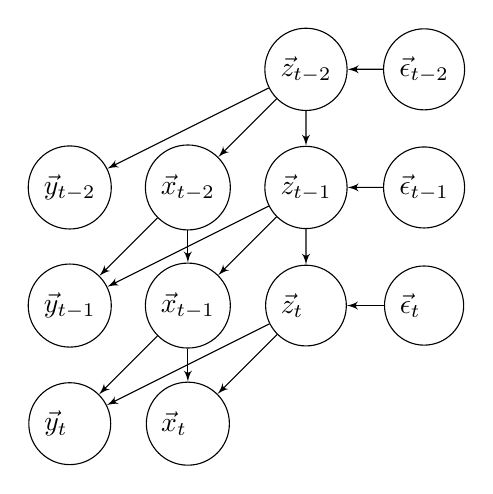
\begin{tikzpicture}[scale=1.5]
          \tikzset{
            vertex/.style={circle,draw, minimum size=2em},
            edge/.style={->,> = latex'}
          }
          % vertices
          \node[vertex] (zt) at (1 ,0) {$\vec{z}_{t\quad}$};
          \node[vertex] (zt1) at (1 , 1) {$\vec{z}_{t-1}$};
          \node[vertex] (zt2) at (1 , 2) {$\vec{z}_{t-2}$};
          \node[vertex] (xt) at (0 ,-1) {$\vec{x}_{t\quad}$};
          \node[vertex] (xt1) at (0 , 0) {$\vec{x}_{t-1}$};
          \node[vertex] (xt2) at (0 , 1) {$\vec{x}_{t-2}$};
          \node[vertex] (yt) at (-1,-1) {$\vec{y}_{t\quad}$};
          \node[vertex] (yt1) at (-1, 0) {$\vec{y}_{t-1}$};
          \node[vertex] (yt2) at (-1, 1) {$\vec{y}_{t-2}$};
          \node[vertex] (et) at (2 , 0) {$\vec{\epsilon}_{t\quad}$};
          \node[vertex] (et1) at (2 , 1) {$\vec{\epsilon}_{t-1}$};
          \node[vertex] (et2) at (2 , 2) {$\vec{\epsilon}_{t-2}$};
      
          %edges
          \draw[edge] (et) -- (zt);
          \draw[edge] (et1) -- (zt1);
          \draw[edge] (et2) -- (zt2);
          \draw[edge] (zt2) -- (zt1);
          \draw[edge] (zt1) -- (zt);
          \draw[edge] (xt2) -- (xt1);
          \draw[edge] (xt1) -- (xt);
          \draw[edge] (zt2) -- (xt2);
          \draw[edge] (zt1) -- (xt1);
          \draw[edge] (zt) -- (xt);
          \draw[edge] (zt2) -- (yt2);
          \draw[edge] (zt1) -- (yt1);
          \draw[edge] (zt) -- (yt);
          \draw[edge] (xt2) -- (yt1);
          \draw[edge] (xt1) -- (yt);
        \end{tikzpicture}
      \end{figure}
\end{frame}

\section{Conclusion}

\begin{frame}
    \frametitle{Github}
    \begin{center}
        \url{https://github.com/e-hall-hoffarth/causal_dsge}
    \end{center}
\end{frame}

\end{document}